\section{Gleichgewichtsensembles}
\begin{tabbing}
Erfahrungsgemäß strebt jedes makroskopische System einem Gleichgewicht zu. $\rightarrow$ Beschreibung des\\ Systems durch ein Ensemble von Mikrozuständen. Messwerte werden als Ensemble-Mittelwerte\\ berechnet.\\
Begründungen:\\
-- \=Messungen benötigen eine gewisse Zeit. In dieser Zeit kann der Mikrozustand durch unvermeidbare\\\> Wechselwirkungen mit der Umgebung geändert werden.\\
-- \= \uline{Erdogenhypothese}: Ein Mikrozustand kommt allen Ensemblezuständen im Laufe der Zeit beliebig\\\> nahe. $\rightarrow$ Ersetze Zeitmittel durch Ensemblemittel.
\end{tabbing}

\subsection{Mikrokanonisches Ensemble}
\label{sec:Mikrokanonisch}
\begin{tabbing}
Bekannt: \= -- \= Form und Energie der Mikrozustände\\
\> -- \> Gesamtenergie liege im Bereich $\edgBra{E,E+\Delta E}$\\
Sei $\Omega$ die Zahl der Zustände in $\edgBra{E,E+\Delta E}$.\\
Maximiere Entropie $\rightarrow$ Gleichverteilung, $P_\nu = \frac{1}{\Omega}$, $S=k_B \ln\Omega$.\\
Mikrokanonisches Ensemble im Phasenraum:\\
Sei $\Omega_{Ph} = \int\limits_{E\leq H\leq E+\Delta E} \prod\limits_j \dd{q}_j\dd{p}_j$ das zugängliche Phasenraumvolumen.\\
\hspace{4em} \= \kill
$\rightarrow$\> Unendlich viele Zustände. Jedoch folgt aus der Quantenmechanik, dass die Zahl der\\\> Mikrozustände $\Omega = \frac{\Omega_{Ph}}{h^{3N}N!}$ ist. ($1$ Mikrozustand \glqq nimmt den Platz $h^{3N}$ ein\grqq, Faktor $N!$\\\> wegen Ununterscheidbarkeit bei $N$ identischen Teilchen.)
\end{tabbing}

\subsection{Temperatur}
\label{sec:Temperatur}
\begin{tabbing}
Betrachte $2$ Systeme $a$, $b$, die Energie austauschen, aber keine Teilchen. Gesamtenergie $E$ sei\\ festgelegt. Wie verteilt sich die Energie auf $a$ und $b$?\\
$E = E_a + E_b$, Zahl der zugänglichen Zustände: $\Omega_a\norBra{E_a}$, $\Omega_b\norBra{E_b}$\\
\hspace{4em} \= \kill
$\rightarrow$\> Gesamtentropie $S = S_a + S_b = S_a\norBra{E_a} + S_b\norBra{E-E_a}$\\
Maximiere Entropie: \= $\ppv{S}{E_a} = 0$\\
\> $\ppv{S_a}{E_a} - \ppv{S_b}{E_b} = 0$\\
\> $\rightarrow$ $\ppv{S_a}{E_a} = \ppv{S_b}{E_b}$\\
\hspace{4em} \= \kill
$\rightarrow$\> Definiere Temperatur eines Systems: \fbox{$T\mDef \norBra{\ppv{S}{E}}^{-1}$}\\
Zwei Systeme sind im \uline{thermischen Gleichgewicht}, wenn die Temperaturen gleich sind ($T_a = T_b$).\\
Temperatur skaliert nicht mit der Systemgröße, sie ist eine \uline{intensive Größe}.
\end{tabbing}

\subsection{Kanonisches Ensemble}
\label{sec:Kanonisch}
\begin{tabbing}
Es sei ein Schätzwert für die Energie bekannt: $\angBra{E}$ festgelegt.\\
\hspace{4em} \= \kill
$\rightarrow$\> Maximiere Entropie $S = -k_B \sum\limits_{\nu} P_{\nu} \ln P_{\nu}$ unter den Nebenbedingungen\\
\> $\sum\limits_\nu P_\nu = 1$\\
\> $\sum\limits_\nu P_\nu E_\nu = \angBra{E}$\\
$\delta\norBra{-\sum\limits_\nu P_\nu \ln\norBra{P_\nu} + lambda\norBra{1-\sum\limits_\nu P_\nu} + \beta\norBra{\angBra{E} - \sum\limits_\nu P_\nu E_\nu}} = 0$\\
Mit Lagrange-Multiplikatoren $\lambda$ und $\beta$\\\
$\rightarrow$\> $\sum\limits_\nu\norBra{\ln\norBra{P_\nu} + 1 + \lambda + \beta E_\nu}\delta P_\nu = 0$, $\delta P_\nu$ können unabhängig gewählt werden\\
Definiere: $\alpha \mDef 1 + \lambda$\\
$\rightarrow$\> $\ln\norBra{P_\nu} + \alpha + \beta E_\nu = 0$ für alle $\nu$\\
$\rightarrow$\> $P_\nu = e^{-\alpha - \beta E_\nu}$\\
Normierung: \= $\sum\limits_\nu P_\nu = \sum\limits_\nu e^{-\alpha-\beta E_\nu} = 1$\\
$\rightarrow$\> $e^\alpha = \sum\limits_\nu e^{-\beta E_\nu}$\\
Definiere \uline{Zustandssumme} \fbox{$Z \mDef \sum\limits_\nu e^{-\beta E_\nu}$}\\
Bestimme $\beta$ über $\angBra{E} = \sum\limits_\nu E_\nu \frac{e^{-\beta EE_\nu}}{Z}$ beziehungsweise \fbox{$\angBra{E} = - \frac{1}{Z} \ppv{Z}{\beta}$}\\
Wahrscheinlichkeitsverteilung: \fbox{$P_\nu = \frac{1}{Z} e^{-\beta E_\nu}$} \uline{Boltzmann-Verteilung}\\
$e^{-\beta E_\nu}$ heißen \uline{Boltzmann-Faktoren}.\\
Wert der Entropie für diese Verteilung:\\
$S$\=$=-k_B \sum\limits_\nu P_\nu \ln\norBra{P_\nu}$\\
\>$=-k_B \sum\limits_ \frac{e^{-\beta E_\nu}}{Z} \ln\norBra{\frac{e^{-\beta E_\nu}}{Z}}$\\
\>$=k_B \sum\limits_\nu \frac{e^{-\beta E_\nu}}{Z} \beta E_\nu + k_B \sum\limits_\nu \frac{e^{-\beta E_\nu}}{Z} \ln Z$\\
\>$=k_B \beta \angBra{E} + k_B \ln Z$; Betrachte $\ppv{S}{\angBra{E}} = k_B \beta + k_B \angBra{E} \ppv{\beta}{\angBra{E}} + k_B \ppv{\ln Z}{\beta} \ppv{\beta}{\angBra{E}}$\\
Definiere $T\mDef \norBra{\ppv{S}{\angBra{E}}}^{-1}$ (analog zu Abschnitt \ref{sec:Temperatur})\\
\hspace{4em} \= \kill
\> $F = -\frac{1}{\beta} \ln Z = - k_B T \ln Z$\\
$\rightarrow$\> $T = \frac{1}{k_B \beta}$, \fbox{$\beta = \frac{1}{k_B T}$}, $S = \frac{\angBra{E}}{T} - \frac{F}{T}$, \fbox{$F = \angBra{E} - T S$}\\
\uwave{Bezeichnungen}: \= $\angBra{E}$ \= innere Energie, auch einfach $E$, $U$\\
\>$T$\> Temperatur\\
\>$F$\> freie Energie, Helmholtz-Energie\\
\>$S$\> Entropie, Clausius-Entropie, Boltzmann-Entropie \\\>\>(Maximalwert der Gibbs-Entropie)\\
\uline{Alternative Herleitung}: \=Mikrokanonisches Ensemble für Gesamtsystem aus System\\\>\> + (großes) Wärmebad
\end{tabbing}


\subsection{Gleichgewicht in der Quantenstatistik}
\begin{tabbing}
Zeitentwicklung der Dichtematrix: $i \hbar \ppv{\rho}{t} = \edgBra{H,\rho}$\\
Gleichgewicht: $\ppv{\rho}{t} = 0$ $\rightarrow$ $\edgBra{H,\rho} \stackrel{!}{=} 0$\\
\uline{Vertauschende} Operatoren besitzen \uline{gemeinsame} Eigenzustände.\\
\hspace{4em} \= \kill
$\rightarrow$\> Energieeigenzustände $\ket{\Phi_j}$ mit $H \ket{\Phi_j} = E_j \ket{\Phi_j}$ sind auch Eigenzustände von $\rho$.\\
$\rightarrow$\> Konstruiere Dichtematrix: $\rho = \sum\limits_j P_j \ket{\Phi_j}\bra{\Phi_j}$\\\> mit $\sum\limits_j P_j = 1$, $\braket{\Phi_j}{\Phi_k} = \delta_{jk}$, $\tr\norBra{\rho\ln\norBra{\rho}} = \sum\limits_j P_j \ln\norBra{P_j}$\\
$\rightarrow$\> Herleitung durch Entropiemaximierung wie in \ref{sec:Mikrokanonisch}, \ref{sec:Kanonisch}\\
Kanonisches Ensemble:\\
\> $\rho = \sum\limits_j \frac{e^{-\beta E_j}}{Z} \ket{\Phi_j}\bra{\Phi_j} = \sum\limits_j \frac{e^{-\beta H}}{Z} \ket{\Phi_j}\bra{\Phi_j}$\\
$\rightarrow$\> \fbox{$\rho = \frac{e^{-\beta H}}{Z}$} wobei $\beta = \frac{1}{k_B T}$, $Z = \sum\limits_j e^{-\beta E_j} = \sum\limits_j \brExpet{\Phi_j}{e^{-\beta H}}{\Phi_j}$\\
$\rightarrow$\> \fbox{$Z = \tr\norBra{e^{-\beta H}}$}\\
Energie: $U = \angBra{H} = \tr\norBra{\rho H} = \frac{1}{Z} \tr\norBra{e^{-\beta H} H} = - \frac{1}{Z} \ppv{Z}{\beta}$ oder $U = - \ppv{}{\beta} \ln Z$\\
\uwave{Beispiel}: \= Ein eindimensionaler harmonischer Oszillator\\
\> $E_j = \hbar\omega \norBra{j + \frac{1}{2}}$\\
\> $Z = \sum\limits_j e^{-\beta E_j} = e^{-\frac{\beta\hbar\omega}{2}} \sum\limits_j e^{-\beta\hbar\omega} = e^{-\frac{\beta\hbar\omega}{2}} \frac{1}{1-e^{-\beta\omega}}$\\
$\angBra{H} = -\ppv{}{\beta}\edgBra{-\frac{\beta\hbar\omega}{2} - \ln\norBra{1 - e^{-\beta\hbar\omega}}} = \frac{\hbar\omega}{2} + \frac{\hbar\omega e^{-\beta\hbar\omega}}{1 - e^{-\beta\hbar\omega}} = \hbar\omega\norBra{\frac12 + \frac{1}{e^{\beta\hbar\omega}}}$
\end{tabbing}


\subsection{Ideales Gas (unterscheidbare Teilchen)}
\begin{tabbing}
Betrachte abgeschlossenes System mit fester Teilchenzahl $N$, festem Volumen $V$, Teilchenmasse $m$.\\
(Begriffe \= \uline{abgeschlossen}, \uline{isoliert} \= -- kein Austausch von Energie oder Materie mit Umgebung\\
\>\uline{geschlossen}\> -- Austausch von Energie, aber kein Austausch von Materie\\
\>\uline{offen}\> -- Austausch von Energie und Materie mit Umgebung)\\
Hamiltonfunktion beziehungsweise -Operator: $H = \sum\limits_{j=1}^{3N} p_j^N + V_\text{Wand}$\\
\uline{Klassisch}: Koordinaten begrenzt durch Volumen $V$, Impulse $-\infty < p_j < \infty$\\
\uline{Quantenmechanisch}: \=nur bestimmte Impulse erlaubt. Eigentlich Potentialtopfzustände, aber Analyse\\\> kann für große Energien durch Verwendung periodischer Randbedingungen\\\> vereinfacht werden. Annahme $V = L^3$ (Würfel).\\
$\rightarrow$\> $\psi\norBra{q_j} \stackrel{!}{=} \psi\norBra{g_j + L}$\\
$\rightarrow$\> Impulse $p_j = \hbar k_j = \hbar \frac{2\pi}{L} n_j$, $j = 1, \dots, 3N$ in Wellenfunktion $\phi \sim \prod\limits_{j=1}^3N e^{i p_j\cdot q_j}$.\\
$\rightarrow$\> $1$ Zustand nimmt das Impulsraumvolumen $\norBra{\frac{2\pi\hbar}{L}}^{3N}$ ein.\\
$\rightarrow$\> In ein Phasenraumvolumen $\Omega_{Ph}$ passen $\frac{\Omega_{Ph}}{h^{3N}}$ Zustände.\\
\> Energien: $E 0 \frac{1}{2 m} \norBra{\frac{2\pi\hbar}{L}}^2 \sum\limits_{j=1}^{3N} n_j^2$
\end{tabbing}
\begin{figure}[H]
  \centering
  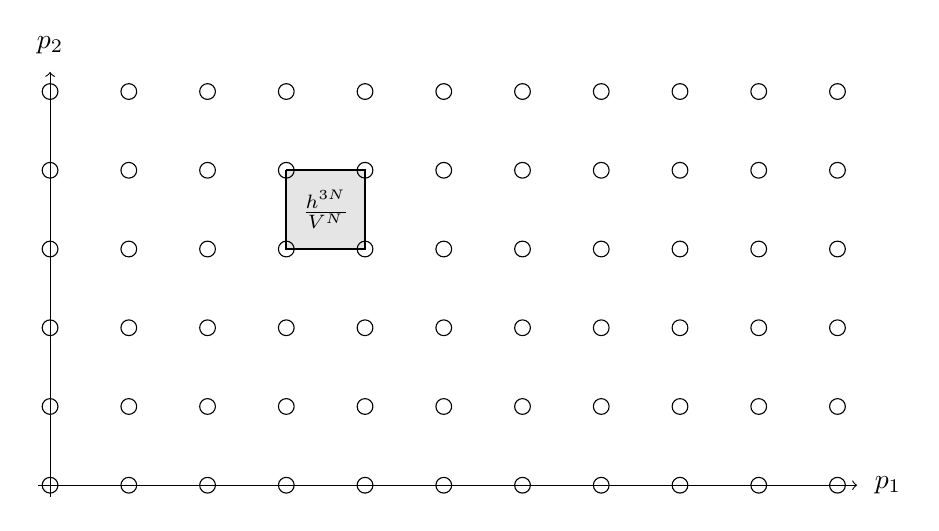
\begin{tikzpicture}
    \draw[->] (-0.15,0) to (10.25,0);
    \draw[->] (0,-0.15) to (0,5.25);
    \node[anchor=west] at (10.35,0) {$p_1$};
    \node[anchor=south] at (0,5.35) {$p_2$};
    \draw[thick,fill=white!90!black] (3,4) to (4,4) to (4,3) to (3,3) to (3,4) ;
    \foreach \x in {0,1,...,10} \foreach \y in {0,1,...,5} \draw (\x,\y) circle (0.1);
    \node at (3.5,3.5) {$\frac{h^{3N}}{V^N}$};
  \end{tikzpicture}
\end{figure}


\subsubsection{Mikrokanonische Behandlung}
\label{sec:Mikbeh}
\begin{tabbing}
Zustände mit Energie $\leq E$ liegen im $3N$-dimensionalen Impulsraum innerhalb einer Kugel mit Radius\\
$R = \sqrt{2 m E}$, Volumen einer $D$-dimensionale Kugel: $K_D = \frac{\pi^{\frac{D}{2}}}{\Gamma\norBra{\frac{D}{2} + 1}} R^D$\\
mit Gammafunktion $\Gamma\norBra{x} = \int\limits_0^\infty t^{x-1} e^{-t} \dd{t}$.\\ Betrachte gerade $D$ $\rightarrow$ $\Gamma\norBra{\frac{D}{2} + 1} = \norBra{\frac{D}{2}}!$\\
\uwave{Gesucht}: \= Anzahl der Zustände mit Energien in $\edgBra{E-\Delta E, E}$\\
\> $\eDef$ Kugelschale mit Dicke $\Delta R \approx \frac{m}{\sqrt{2 m E}}\cdot \Delta$\\
\> $\eDef$ Volumen $\ppv{K_D}{R}\cdot \Delta R = \frac{D\cdot K_D}{R}\cdot \Delta R = \vcentcolon \Delta K_D$\\
\> $\frac{\Delta K_D}{K_D} = D \frac{\Delta R}{R}$, das heißt für $D = 3N \to \infty$ liegt fast das ganze Kugelvolumen am Rand!\\
$\rightarrow$\> $\Delta K_D \approx K_D$\\
$\rightarrow$\> Anzahl der Zustände: $\Omega = \frac{K_{3N}V^N}{h^{3N}} = \frac{\pi^{\frac{3N}{2}}}{\norBra{\frac{3N}{2}}!} \norBra{2 m E}^{\frac{3 N}{2}}\frac{V^N}{h^{3N}}$\\
Entropie: $S = k_B \ln \Omega$\\
Verwende Stirling-Formel $\ln\norBra{\norBra{\frac{3N}{2}}!} \stackrel[N\to\infty]{}{=} \frac{3N}{2} \ln\norBra{\frac{3N}{2}} - \frac{3N}{2}$\\
$\rightarrow$\> $S = k_B \ln\norBra{\norBra{2\pi m E}^{\frac{3 N}{2}}\frac{V^N}{h^{3N}}} - k_B \cdot \frac{3N}{2} \ln\norBra{\frac{3 N}{2}} + k_B \cdot\frac{3N}{2}$\\
\> \fbox{$S = k_B N \ln \edgBra{\norBra{\frac{4 \pi m}{3 h^2}}^{\frac32}\norBra{\frac{E}{N}}^{\frac32}V}$}\\
$\rightarrow$\>$E = \frac{3h^2}{4\pi m} \frac{N}{V^{\frac32}} e^{\frac{2 S}{3 k_B N} - 1}$ Innere Energie\\
$T^{-1} = \ppv{S}{E} = \ppv{}{E}\norBra{k_B N \ln\norBra{E^{\frac32}}} = k_B N \cdot \frac32 \frac{1}{E}$\\
$\rightarrow$\> \fbox{$E = \frac32 k_B T$}\\
$N=\text{Teilchenzahl} = \text{Molzahl}\cdot \frac{R}{k_B}$ $\rightarrow$ $E = \frac32 n R T$.\\
\uline{Wärmekapazität}: $C \mDef \left. \ppv{E}{T}\right\rvert_{N,V} = \frac32 N k_B$\\
Anscchaulich: Jedes Teilchen trägt mittlere Energie $\frac32 k_B T$\\
Dies ist ein Spezialfall des \uline{Äquipartitionstheorems}, welches besagt, dass ein Freiheitsgrad, der\\ quadratisch in die Hamiltonfunktion eingeht (hier jede Impulskomponente) im Gleichgewicht und bei\\ hohen Temperaturen die Energie $\frac{k_B T}{2}$ trägt.
\end{tabbing}

\subsubsection{Kanonische Behandlung}
\label{sec:Kanbeh}
\begin{tabbing}
Impulse $p_1, \dots ,p_{3N}$ $\rightarrow$ Energie $E = \sum\limits_{j=1}^{3N} \frac{p_j^2}{2 m}$\\
Boltzmannverteilung: $P\norBra{E} = \frac{e^{-\beta E}}{Z}$\\
mit \=$Z = \sum e^{-\beta E} = \int \prod\limits_j \dd{q_j}\dd{p_j} \frac{1}{h^{3N}} e^{-\beta\frac{\norBra{p_1^2 + \dots + p_{3N}^2}}{2 m}}$\\
$\rightarrow$\> $Z = Z_1^{3N}$ mit $Z_1 = \int\dd{q}\int\limits_{-\infty}^\infty \dd{p} \frac{1}{h} e^{-\beta\frac{p^2}{2 m}} = \frac{L}{h} \sqrt{2\pi m k_B T}$\\
Entropie: $S = k_B \beta \angBra{E} + k_B \ln Z$\\
mit $\angBra{E}=-\ppv{}{\beta} \ln Z=-3N \ppv{}{\beta} \ln Z_1=-3N \ppv{}{\beta} \ln \sqrt{\frac{1}{\beta}}=\frac32 N \ppv{}{\beta}\ln\beta=\frac32 N \frac{1}{\beta}$\\
\hspace{4em} \= \kill
$\rightarrow$\> \fbox{$\angBra{E} = \frac32 N k_B T$}\\
$\rightarrow$\> $S = \frac32 N k_B + k_B \ln Z = \frac32 N k_B + 3 N k_B \ln\norBra{\sqrt{2\pi m k_B T}\frac{L}{h}}$\\
$\rightarrow$\> \fbox{$S = \frac32 N k_B + N k_B \ln\edgBra{\frac{V}{h^3}\norBra{2\pi m k_B T}^{\frac32}}$}\\
(identisch zum Ergebnis beim mikrokanonischen Ensemble)\\
Beachte: \=Für diesen Ausdruck gilt $S\stackrel[T\to 0]{}{\to} -\infty$, Widerspruch zur Definition der Entropie ($S\geq 0$).\\\> Grund: Einteilung des Phasenraums in volumina $h^{3N}$ ist nur bei großen Temperaturen\\\> (klassischer Limes) richtig.
\end{tabbing}

\subsubsection{Gibbsches Paradoxon}
\begin{tabbing}
Entropie $S$ muss eine extensive Größe sein, das heißt bei Skalierung der Systemgröße\\
$N \to\alpha N$, $V\to \alpha V$ muss gelten $S\to\alpha S$.\\
Für die Entropie in \ref{sec:Kanbeh}, \ref{sec:Mikbeh} gilt jedoch:\\
\hspace{4em} \= \kill
\> $S \to \alpha S + \alpha N k_B \ln \alpha$ ($N = \text{Teilchenzahl}$)\\
$\rightarrow$\> Beim Zusammenführen zweier Gase zu einem neuen System gibt es eine \uline{Mischentropie}\\\> (\glqq Zunahme der Unordnung\grqq )\\
Erklärung: \= -- Teilchen wurden als unterscheidbar angenommen.\\
\> -- Mischentropie ist sinnvoll beim Mischen verschiedener Gase:
\end{tabbing}
\begin{figure}[H]
  \centering
  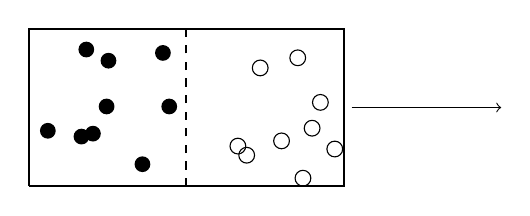
\begin{tikzpicture}
  \draw[thick] (0,0) to (4,0) to (4,2) to (0,2) to (0,0);
  \draw[thick,dashed] (2,0) to (2,2);
  \pgfmathsetseed{3}
  \foreach \x in {1,...,9} \fill (rand*0.9+1,rand*0.9+1) circle (0.1);
  \foreach \x in {1,...,9} \draw (rand*0.9+3,rand*0.9+1) circle (0.1);
  \draw[->] (4.1,1) to (6,1);
  \end{tikzpicture}
  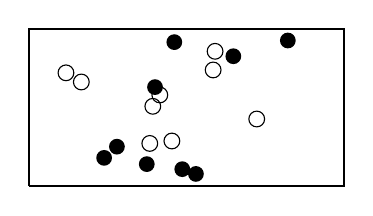
\begin{tikzpicture}
  \draw[thick] (0,0) to (4,0) to (4,2) to (0,2) to (0,0);
  % \pgfmathsetseed{4}
  \foreach \x in {1,...,9} \fill (rand*1.8+2,rand*0.9+1) circle (0.1);
  \foreach \x in {1,...,9} \draw (rand*1.8+2,rand*0.9+1) circle (0.1);
  \end{tikzpicture}
\end{figure}
\begin{tabbing}
Bei gleichen Gasen darf es keine Mischentropie geben.\\
\hspace{4em} \= \kill
$\rightarrow$\> Korrektur der Anzahl der Zustände: $\Omega \to \frac{1}{N!} \Omega$,$Z \to \frac{1}{N!}Z$\\
$N!$ berücksichtigt die Ununterscheidbarkeit im Fall, dass alle Teilchen \uline{verschiedene} Einteilchenzustände\\ ($\vec{p}_1,\dots,\vec{p}_N$) besetzen, also bei genügend hohen Temperaturen.\\
$\rightarrow$\> $Z = \frac{V^N}{N!h^{3N}} \sqrt{2\pi m k_B T}^{3N}$, $\angBra{E} = \frac32 N k_B T$\\
\> $S = k_B \beta \angBra{E} + k_B \ln Z = \frac32 N k_B + k_B \ln\norBra{\frac{V^N}{h^{3N}}\sqrt{2\pi m k_B T}^{3N}} - k_B \ln\norBra{N!}$\\
Stirling $\rightarrow$\> $-k_B \ln\norBra{N!} \approx - k_B N \ln\norBra{N} + k_B N$\\
$\rightarrow$\> \fbox{$S = \frac52 N k_B + N k_B \ln \edgBra{\norBra{\frac{V}{N}}\frac{1}{h^3}\sqrt{2\pi m k_B T}^3}$} \uline{extensiv}
\end{tabbing}


\subsection{Äquipartitionstheorem und Virialsatz}
\begin{tabbing}
Klassisches System mit Phasenraumvariablen $x_j$ ($q_j$ oder $p_j$) und Hamiltonfunktion $H = \sum\limits_n \sum\limits_{j=1}^f a_{j,n} x_j^n$;\\
Verwende kanonisches Ensemble.\\
Betrachte $\angBra{x_j \ppv{H}{x_k}} = \frac{1}{Z_{Ph}}\int e^{-\beta H} x_j \ppv{H}{x_k} \dd{\Gamma}$, $Z_{Ph} = \int e^{-\beta H} \dd{\Gamma}$\\
$\angBra{x_j \ppv{H}{x_k}} = - \frac{1}{\beta Z_{Ph}} \int x_j \ppv{e^{-\beta H}}{x_k} \dd{\Gamma} = - \frac{1}{\beta Z_{Ph}}\edgBra{\int \ppv{}{x_k} \norBra{x_j e^{-\beta H}}\dd{\Gamma} - \int \delta_{jk}e^{-\beta H} \dd{\Gamma}}$\\
Gauß: $\int \ppv{}{x_k} \norBra{x_j e^{-\beta H}}\dd{\Gamma} = \oint x_j e^{-\beta H} \vec{e_k}\cdot \vec{\dd{A}} = 0$, falls $e^{-\beta H} \to 0$ genügend schnell.\\
Dies ist insbesondere erfüllt für $n=2$.\\
\hspace{4em} \= \kill
$\rightarrow$\> $\angBra{x_j \ppv{H}{x_k}} = \frac{1}{\beta Z_{Ph}} \delta_{jk} \int e^{-\beta H} \dd{\Gamma} = k_B T \delta_{jk}$\\
$\rightarrow$\> \fbox{$\angBra{x_j\ppv{H}{x_k}} 0 k_B T \delta_{jk}$} \uline{allgemeines Äquipartitionstheorem}\\
Ideales Gas: $H = \sum\limits_{j=1}^{3N} \frac{p_j^2}{2 m}$, $\angBra{p_j\ppv{H}{p_j}} = 2\cdot \angBra{\frac{p_j^2}{2 m}} = k_B T$\\
$\rightarrow$\> $\angBra{\frac{p_j^2}{2 m}} = \frac{k_B T}{2}$\\
Allgemeiner: \=$H = \sum\limits_{j=1}^{3N} \frac{p_j^2}{2 m} + V$\\
\> $\sum\limits_j \angBra{p_j\ppv{H}{p_j}} = 2 \angBra{E_{kin}} = 3 N k_B T$\\
\> $\sum\limits_j \angBra{q_j\ppv{H}{q_j}} = \sum\limits_j \angBra{q_j\ppv{H}{q_j}} = 3 N k_B T$\\
$\rightarrow$\> \fbox{$\angBra{E_{kin}} = \frac12 \sum\limits_j \angBra{q_j\ppv{H}{q_j}} = -\frac12 \sum\limits_j\angBra{q_j F_j}$} (\uline{Virialsatz})\\
Für jeden Freiheitsgrad, der quadratisch in die Hamiltonfunktion eingeht (kinetische Energie $\frac{p_j^2}{2 m}$ oder\\
harmonisches Potential $\frac12 k q_j^2$), erhält man die mittlere Energie $\frac{k_B T}{2}$.\\
Dies gilt \uline{nicht} in Quantensystemen, zum Beispiel harmonischer Oszillator:\\
\hspace{4em} \= \kill
\>$\angBra{H} = \hbar\omega\norBra{\frac12 + \frac{1}{e^{-\beta \hbar\omega}-1}} \approx \left\{ \begin{array}{r@{\quad , \quad} l}\frac{\hbar\omega}{2} + \hbar\omega e^{-\beta\hbar\omega}\approx \frac{\hbar\omega}{2} & T\to 0\\ \frac{\hbar\omega}{2} + k_B T \approx k_B T & T\to\infty\end{array}\right.$\\
Für große $T$: \=Äquipartitionstheorem gültig\\
Für kleine $T$:\> Freiheitsgrade sind \glqq eingefroren\grqq.\\
Virialsatz ist auch quantenmechanisch gültig, zum Beispiel Teilchen im Coulombpotential:\\
$H = \frac{\vec{p}^2}{2 m} - \frac{1}{4\pi \epsilon_0 \verBra{\vec{r}}}$, $2\angBra{E_{kin}} = - \angBra{E_{Pot}}$.
\end{tabbing}


\subsection{Großkanonisches Ensemble}
\begin{tabbing}
Betrachte offenes System; keine feste Teilchenzahl, aber Erwartungswert $\angBra{N}$ sei vorgegeben.\\
\uwave{Beispiele}: Flüssigkeit $+$ Dampf, Hohlraum mit Wärmestrahlung, chemische Reaktionen\\
Nebenbedingungen für Wahrscheinlichkeiten $P_j$:\\
$\sum\limits_j P_j = 1$, $\sum\limits_j P_j E_j = \angBra{E}$, $\sum\limits_j P_j N_j = \angBra{N}$\\
\hspace{4em} \= \kill
$\rightarrow$\> $3$ Lagrangemultiplikatoren $\alpha$, $\beta$, $\gamma$\\
$\rightarrow$\> Wahrscheinlichkeiten $P_j = e^{-\alpha-\beta E_j - \gamma N_j}$\\
$\sum\limits_j P_j = 1$ $\rightarrow$ $e^{\alpha} = \sum\limits_j e^{-\beta E_j - \gamma N_j} = \vcentcolon Z_G$ (\uline{großkanonische Zustandssumme})\\
Definiere $\mu \mDef - \frac{\gamma}{\beta}$ \uline{chemisches Potential}\\
$\rightarrow$\> \fbox{$P_j = \frac{1}{Z_G} e^{-\beta\norBra{E_j - \mu N_j}}$}, \fbox{$Z_G = \sum\limits_j e^{-\beta\norBra{E_j - \mu N_j}}$} mit $\beta = \frac{1}{k_BT}$\\
(Bei mehreren Teilchensorten können mehrere Nebenbedingungen $\angBra{N_A}$, $\angBra{N_B}$, \dots spezifiziert werden.\\
$\rightarrow$ Mehrere $\mu_a$, $\mu_B$, \dots)\\
\uline{Großkanonische Entropie}:\\
\> $S_G = -k_B \sum\limits_j P_j \ln\norBra{P_j} = k_B \sum\limits_j \frac{e^{-\beta\norBra{E_j - \mu N_j}}}{Z_G} \beta \norBra{E_j - \mu N_j} + k_B \sum\limits_j \frac{e^{-\beta\norBra{E_j - \mu N_j}}}{Z_G} \cdot \ln\norBra{Z_G}$\\
$\rightarrow$\> $S_G = k_B \beta \angBra{E-\mu N} + k_B \ln\norBra{Z_G}$\\
Definiere großkanonisches Potential: \fbox{$\Phi \mDef k_B T \ln\norBra{Z_G}$}\\
$\rightarrow$\> $\Phi = \angBra{E} - T S_G - \mu \angBra{N}$ (analog zur freien Energie beim kanonischen Ensemble)
\end{tabbing}
